\documentclass{beamer}

\usepackage{graphicx}	% allows you to include pictures
\usepackage{default}
%\usepackage{Backstage}
%\usetheme{Bergen}
%\usetheme{AnnArbor}	% There are many other themes available
%\usetheme{Madrid}

%\title[Short Title]{The longer version of the title}
%\AtBeginSection[]{
%\begin{frame}<beamer>{Outline}
% \tableofcontents[currentsection,currentsubsection]
%\end{frame}
%}


\begin{document}
\begin{frame}
\frametitle{Sample Slide}
Here is a formula
\[
 \int_{-\infty}^{\infty}e^{-x^2} \, dx = \sqrt{\pi}.
\]
Here is an itemized list:
\begin{itemize}
\item<2-> First Item
\item[3-] Second Item
\item[4-] Third Item
\end{itemize}

\end{frame}

\begin{frame}{Include a Picture}
\begin{theorem}
 True statement goes here.
\end{theorem}
\begin{center}
 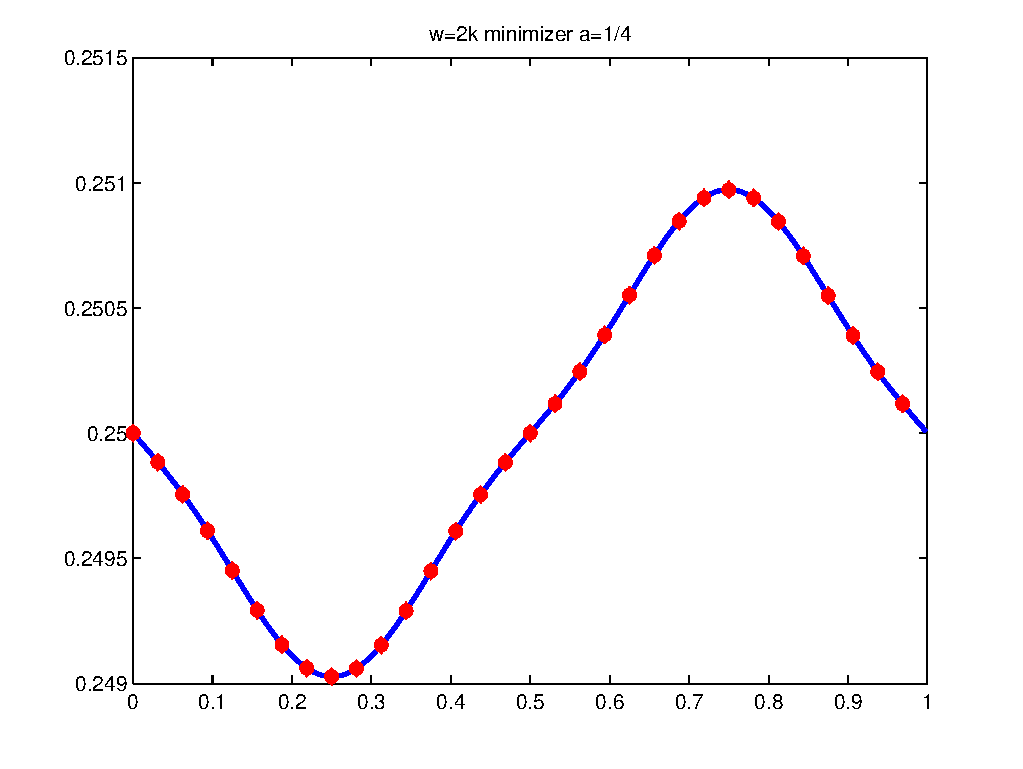
\includegraphics[height=1.5in]{sample.pdf} % if you include a .pdf graphic then compile with pdflatex
\end{center}
\end{frame}

\section{Introduction}

\begin{frame}{Talk Outline}
\uncover<1->{
  \begin{itemize}
    \item<2-> Introduce the background material and basic ideas.
    \item<3-> Explain the main result.
    \item<4-> Show some applications.
  \end{itemize}
}
\uncover<5->{
  \begin{itemize}
    \item<6-> Mention future work and possible
	      extensions of this result.
  \end{itemize}
}
\end{frame}
\end{document}